\documentclass[aspectratio=169]{beamer}              % only frames

% for themes, etc.
\mode<presentation>
\usetheme{Madrid} 
\usecolortheme{crane}

%\usepackage{times}  % fonts are up to you
% The usual suspects
\usepackage{multirow, booktabs, dcolumn, color, graphicx} % Tables\usepackage{graphicx}
\usepackage{amsmath,amssymb,amsthm}
% Strikethrough text
\usepackage{soul}
% Adjust box to fit tabulars
\usepackage{adjustbox}
% Embed video
\usepackage{media9}
% For notes
\usepackage{pgfpages}
%\setbeameroption{hide notes} % Only slides
%\setbeameroption{show only notes} % Only notes
\setbeameroption{hide notes} % Both
% Give a slight yellow tint to the notes page
%\setbeamertemplate{note page}{\pagecolor{yellow!5}\insertnote}\usepackage{palatino}
% Use colors by name
\usepackage{xcolor}
% EMBEDDING VIDEO IS POSSIBLE WITH PDFPC USE PDF PC to present
\usepackage{multimedia}



% The table highlighting for hypothesis discussion.
\usepackage[beamer,customcolors]{hf-tikz}
\usetikzlibrary{calc}

% To use background images
\newenvironment{colorframe}[2][]{%
\setbeamercolor{background canvas}{bg=#1}
\begin{frame}\color{white}}
{\end{frame}}


% To set the hypothesis highlighting boxes red.
\tikzset{hl/.style={
    set fill color=red!80!black!40,
    set border color=red!80!black,
  },
}

% Set Graphics folder
\graphicspath{{./figures/}}


% these will be used later in the title page
\title{Computer Networks}
\subtitle{Root of All Evil Edition}
\author{Irfan Kanat}
\institute[CBS]{{Department of Digitization}\\ Copenhagen Business School}
\date{\today}



\begin{document}

% this prints title, author etc. info from above
\begin{frame}

	\titlepage

\end{frame}

\note{Lets talk about computer networks over a simplified example.

We will learn about various forms of addressing that is used to route packages in a modern network.}



\begin{frame}
	\frametitle{A Tale of Two Computers}

	% EXPLAIN TO THE STUDENTS THAT YOU WILL EXPLAIN BASICS OF COMPUTER NETWORKING
	% THROUGH A SERIES OF INCREASINGLY MORE COMPLEX SITUATIONS
	\centering
	% You have two computers you want to connect
	\only<1>{
\includegraphics[width = \textwidth, height = .85\textheight, keepaspectratio]{figures/2Computers.png}}
	% Simplest solution is to just connect the two with a wire
	\only<2>{
\includegraphics[width = \textwidth, height = .85\textheight, keepaspectratio]{figures/2ComputersCable.png}}
	% You hard code the functionality for the two to talk and you are a happy camper!
\end{frame}


\note{This and the following slides are increasingly complex situations that explain how networks work.

If you want data to go from one computer to the other, simplest solution is to connect them with a wire (Ethernet cable maybe).

}


\begin{frame}
	\frametitle{A Tale of More Computers}
	\centering

	% What if you had more computers?
	\only<1>{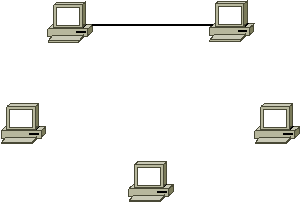
\includegraphics[width = \textwidth, height = .85\textheight, keepaspectratio]{figures/5Computers.png}}
    % Do you see a problem with the same approach?
    \only<2>{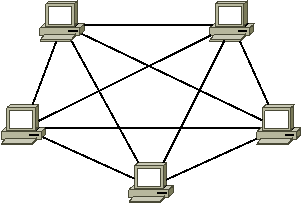
\includegraphics[width = \textwidth, height = .85\textheight, keepaspectratio]{figures/5ComputersCables.png} }
    % I mean besides the obvious infernal infestation angle
    % Do you want demons to possess your network?!?
    % Cause this is how you get demonic possession
    \only<3>{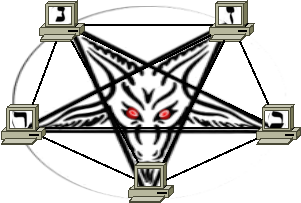
\includegraphics[width = \textwidth, height = .85\textheight, keepaspectratio]{figures/5ComputersInfernal.png} }
    % Tying 5 computers together in a pentagram
    % The packages traversing the network awaken the ancient power symbols
    % and our dark lord baphomet enters your network. FOOOL!

\end{frame}


\note{
	Do you see a problem with this approach?

	I mean besides the obvious infernal infestation angle
    Do you want demons to possess your network?!?
    Cause this is how you get demonic possession.
    The packages circling the pentagram network summon Baphomet.
    Remember that ransomware incident last year... yeah.

	There is the obvious cable and network interface costs associated with connecting all computers to all others.

	What if more computers are added? How will we handle it?}

	%The reason writing the whole communication protocol is a bad idea is that scalability will be limited. Not just in terms of number of nodes, but also in terms of technologies. What if we get computers of different sorts? What if we need to connect with different medium (Fiber Optic, Wireless, Coaxial)? 


\begin{frame}
	\frametitle{A Tale of More Computers}

	It gets exponentially harder to scale \vspace{1em}

	$Connections = \frac{N \times (N-1)}{2}$ \vspace{1em}

	Cable and Network interface costs\ldots \vspace{1em}

	General chaos... Not good.

\end{frame}





\begin{frame}
	\frametitle{A Switch Comes to Town - Data Link}

	% NOW YOU HAVE A NETWORK IN THE MOST COMMON SENSE OF THE WORD

    \begin{columns}
		\begin{column}{0.5\textwidth}

		Like a post office \vspace{1em}

		We need addresses \vspace{1em}

		MAC F4:93:7F:E8:58:E3 \vspace{1em}
	
		\end{column}

		\begin{column}{0.5\textwidth}
			\centering
			\only<1>{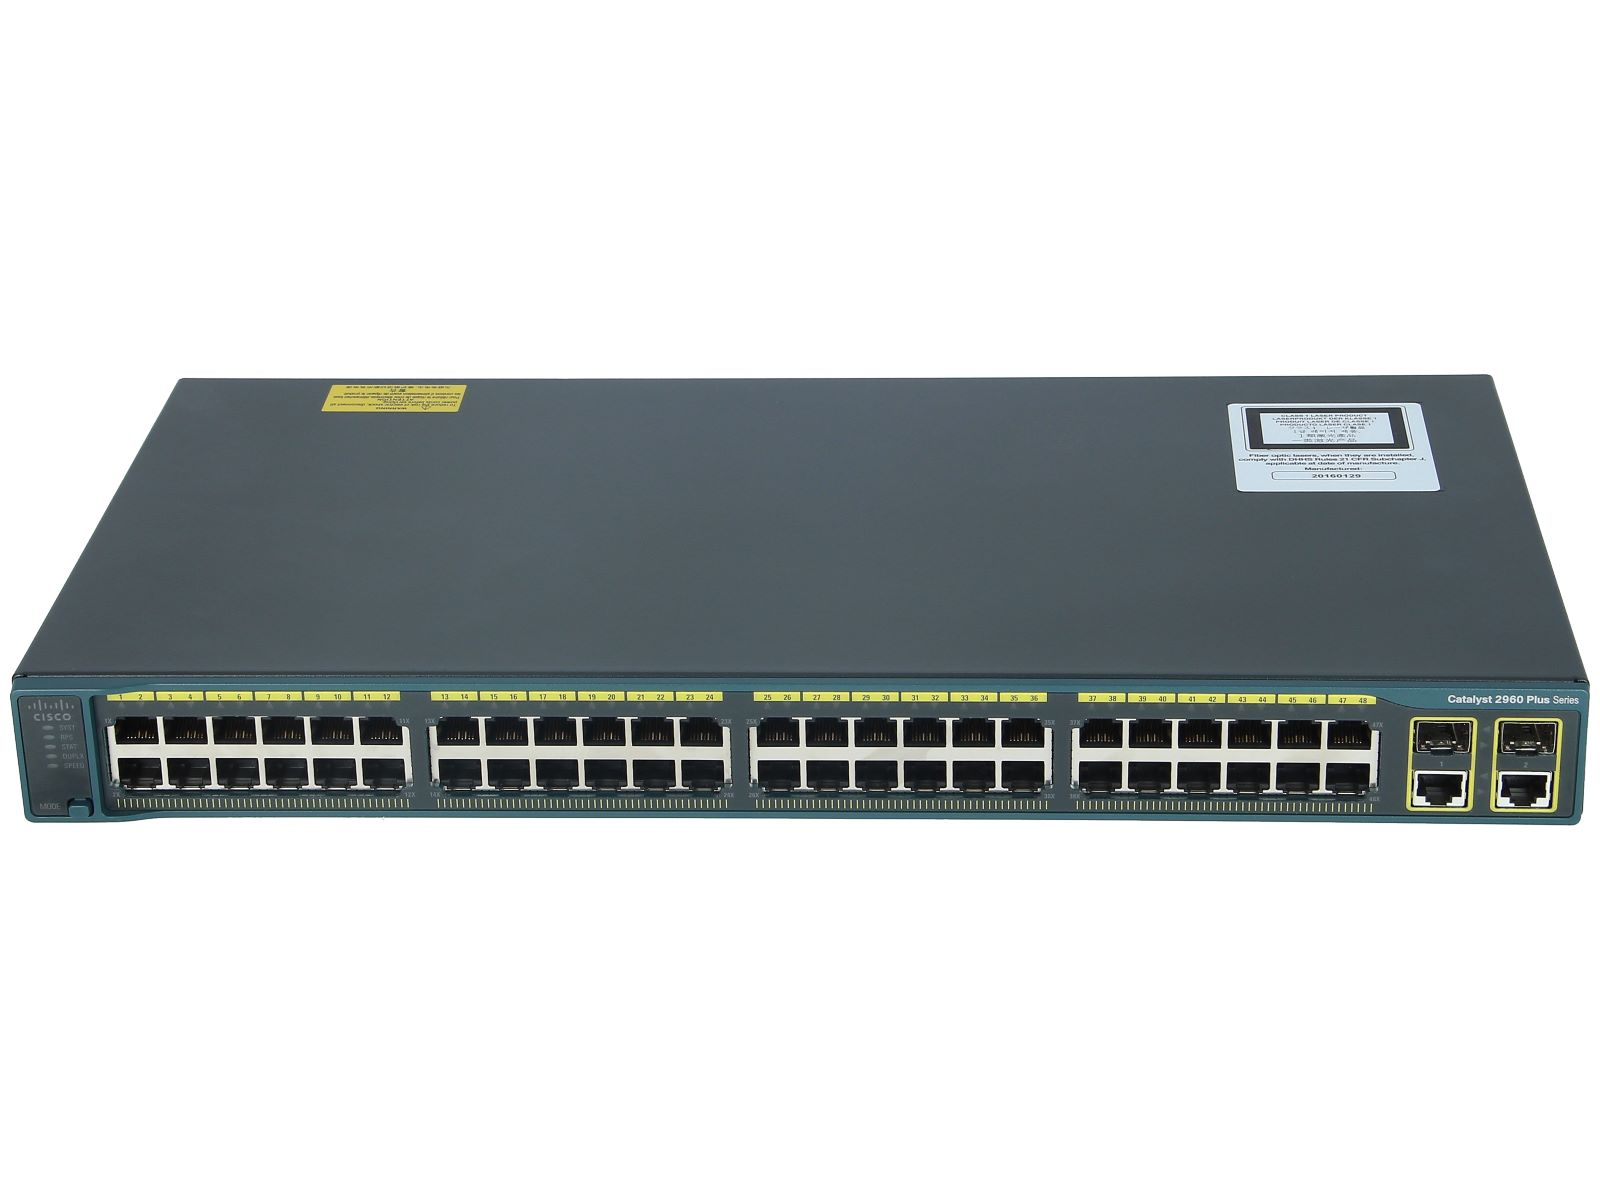
\includegraphics[width = \textwidth, height = .85\textheight, keepaspectratio]{figures/switch.jpg}}
			\only<2>{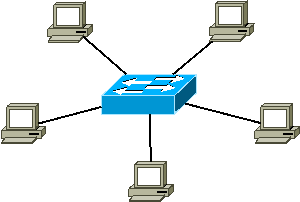
\includegraphics[width = \textwidth, height = .85\textheight, keepaspectratio]{figures/LAN.png}}
			\only<3>{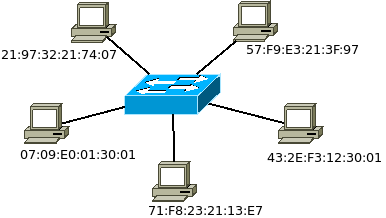
\includegraphics[width = \textwidth, height = .85\textheight, keepaspectratio]{figures/LANMAC.png}}

		\end{column}

	\end{columns}
    
\end{frame}


\note{
With a switch you can form an actually useful network (not like just wiring computers to each other).

A switch is like a post office.

It can deliver data between nodes directly connected to it.

What we need is a way to address each node. The switch will track which node is connected to which wire and send the data to proper nodes.

That is where Physical or MAC addresses come in.

MAC addresses are assigned in the factory. They are static. So unless you spoof your mac address you can't change it.

Fun fact, you can find out the device manufacturer by looking up MAC address.}


\begin{frame}
	\frametitle{When Two Networks Collide - Internet Protocol}
	\centering
	% What if we had two networks of dissimilar computers?
	% One is an ethernet network and the other is cellular phones?
	% Now we need more addresses
	\only<1>{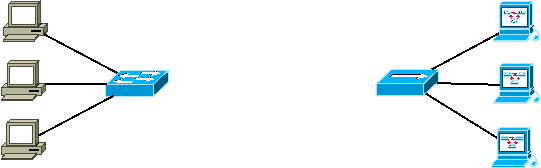
\includegraphics[width = \textwidth, height = .85\textheight, keepaspectratio]{figures/2LANs.png} }

	\only<2>{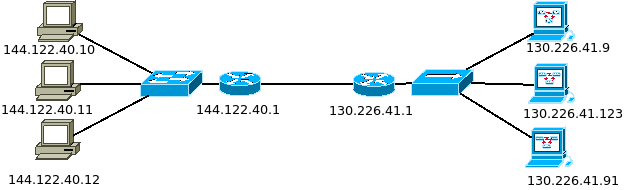
\includegraphics[width = \textwidth, height = .85\textheight, keepaspectratio]{figures/2LANsIP.png} }
    

\end{frame}


\note{Since I am a sadistic bastard, I want to make your life more miserable. 

One way to do that is to consider the situation where nodes are not in the same network.

The MAC addresses will no longer be useful (there are gazillions of them), and we can't know the physical location of each device.

Here is where IP addressing comes in. The IP addresses are assigned hierarchically. Thus you can estimate where a node will be.}


\begin{frame}
	\frametitle{IP Addressing}

    \begin{columns}
		\begin{column}{0.5\textwidth}

			IP address \vspace{1em}

			\textcolor{orange}{Prefix:} A Network 

		    \textcolor{red}{Suffix:} A Node \vspace{1em}

		    \colorbox{orange}{144.122.98.}\colorbox{red}{32}
	
		\end{column}

		\begin{column}{0.5\textwidth}
			\centering
			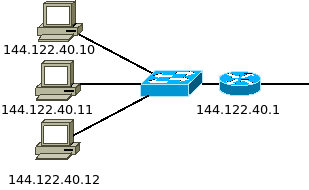
\includegraphics[width = \textwidth, height = .85\textheight, keepaspectratio]{figures/2LANsIPHalf.png}

		\end{column}

	\end{columns}

\end{frame}


\note{
	IP addresses indicate both the network and the specific node in a network.

	IP addresses are 32 binary bits. Usually first so many bits specify the network prefix.

	For the sake of simplicity I am not going into details such as subnet masks. 

	Just know that IP address allow you to identify a network (through prefix) and a node in that network (suffix)

}


\begin{colorframe}[black]

	\centering
	\Large
	Why do we need IP addresses?

\end{colorframe}

\note{
	MAC addresses are static.

	If you had to keep track of all nodes with these static addresses, the forwarding/routing tables would grow huge.

	IP addresses are dynamic. They get assigned when you join a network. They are a bit like zip codes. They are hierarchically organized into networks. So to forward to next hop, all you need to know is general direction the network lies in.

}


{
\usebackgroundtemplate{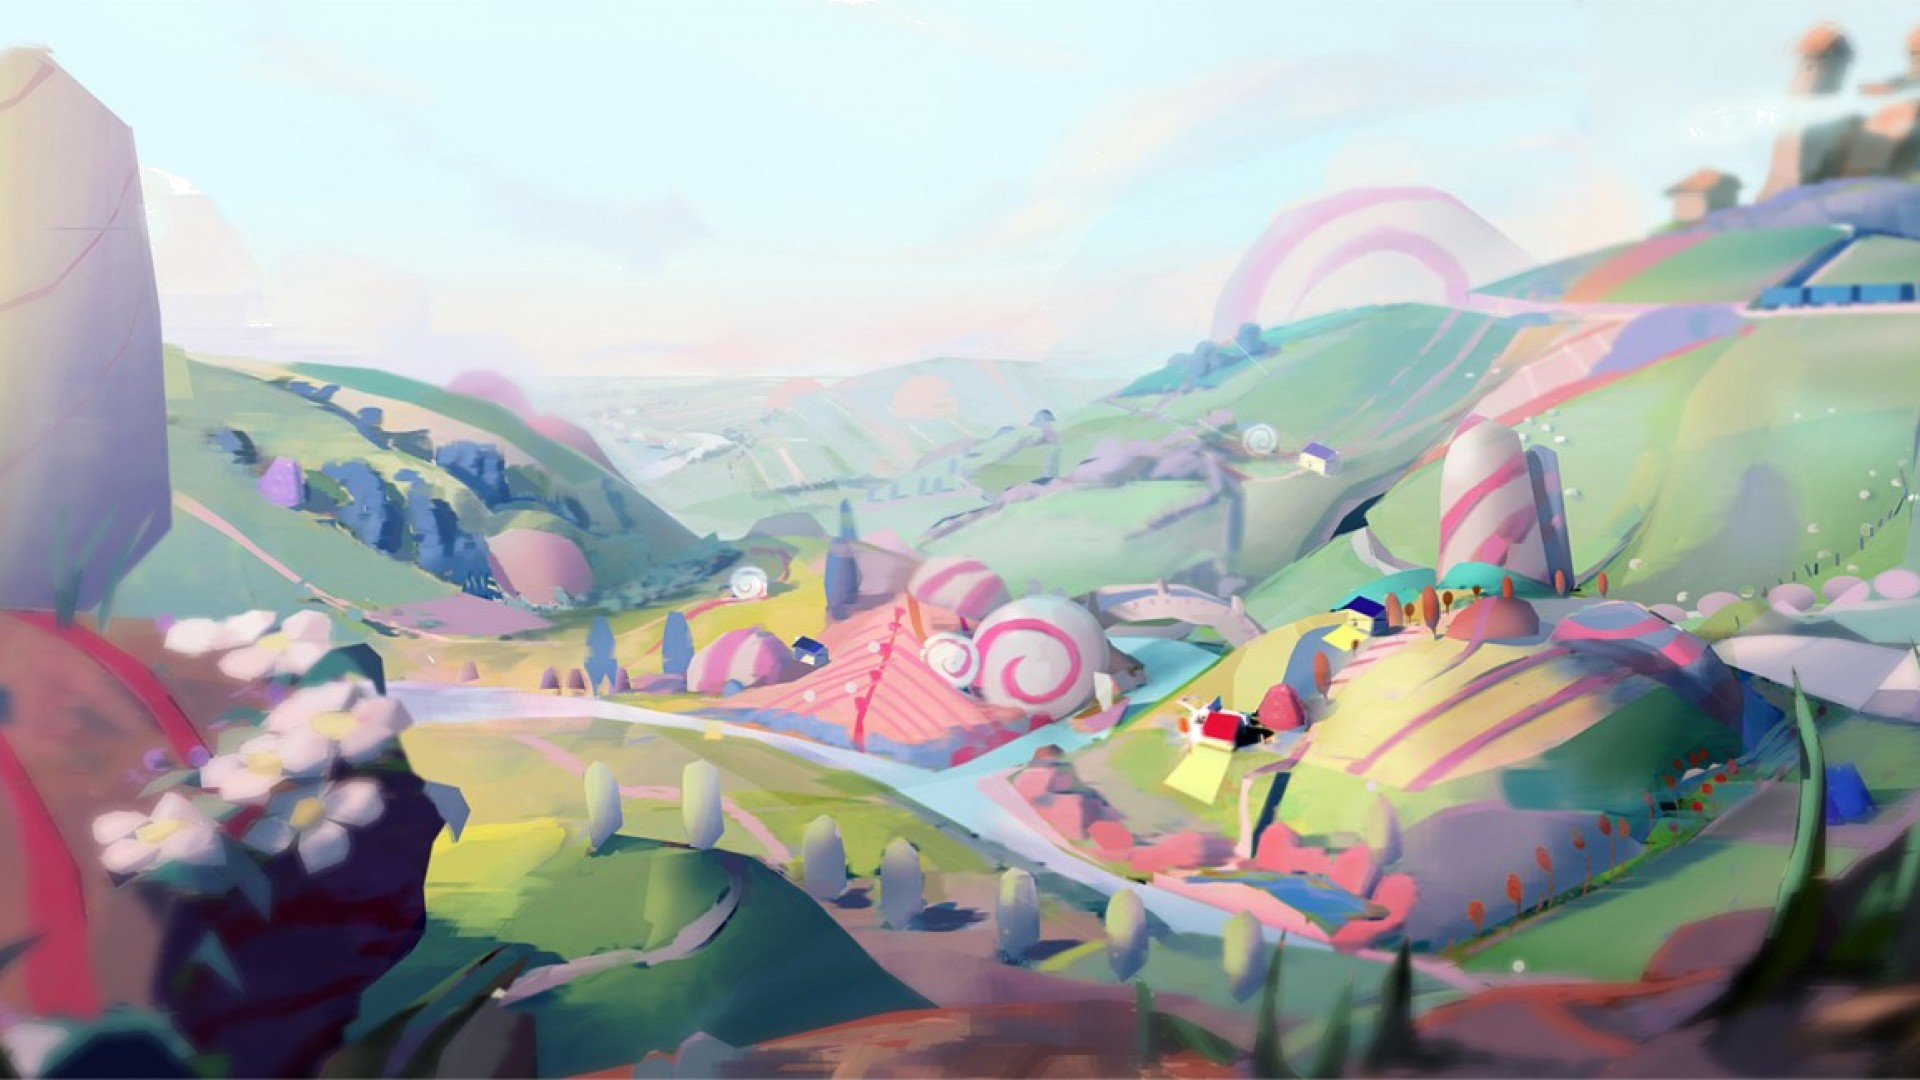
\includegraphics[width=\paperwidth,height=\paperheight]{demoland.png}}%
	\begin{frame}
	\frametitle{VPN and Geolocation}



	\end{frame}
}

\note{Set up a VPN (easiest way is to use builtin opera vpn) then locate your device.

https://www.iplocation.net/find-ip-address}


\begin{frame}
	\frametitle{Each Computer Can Do So Many Wonderous Things!}

	% What if the computers did more than just do one thing?
	% Reading e-mail, watching netflix, browsing the web...
	% How will the computer know which application gets the data?

	% GUESS WHAT WE NEED?
	% YES. MORE ADDRESSES...

	% Each application gets a port address
	\centering
	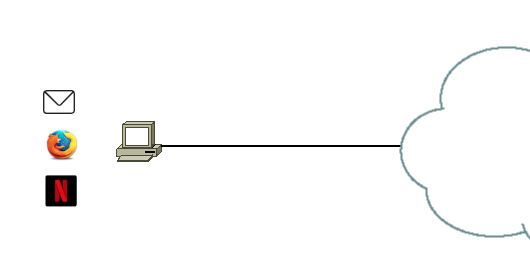
\includegraphics[width = \textwidth, height = .85\textheight, keepaspectratio]{figures/ApplicationLayer.png}
    
\end{frame}

\note{
	OK so we finally managed to get data to the computer where it is needed.

	What if the computers did more than just one thing?
	Reading e-mail, watching netflix, browsing the web...
	How will the computer know which application gets the data?

	GUESS WHAT WE NEED?
	YES. MORE ADDRESSES...

	Each application gets a port address}


\begin{frame}
	\frametitle{Envelopes within envelopes...}

	\centering
    
  	\includegraphics<1>[width = \textwidth, height = .85\textheight, keepaspectratio]{figures/f1-4.png}

   	\includegraphics<2>[width = \textwidth, height = .85\textheight, keepaspectratio]{figures/envelopes.png}

\end{frame}

\note{
	Any time your computer sends or receives data from the network, it comes in multiple envelopes.

	Each layer of the stack receives the data from the layer above, puts in the layer specific addressing and passes it on.

	When determining where a package needs to go, the network uses these addresses.
}


{
\usebackgroundtemplate{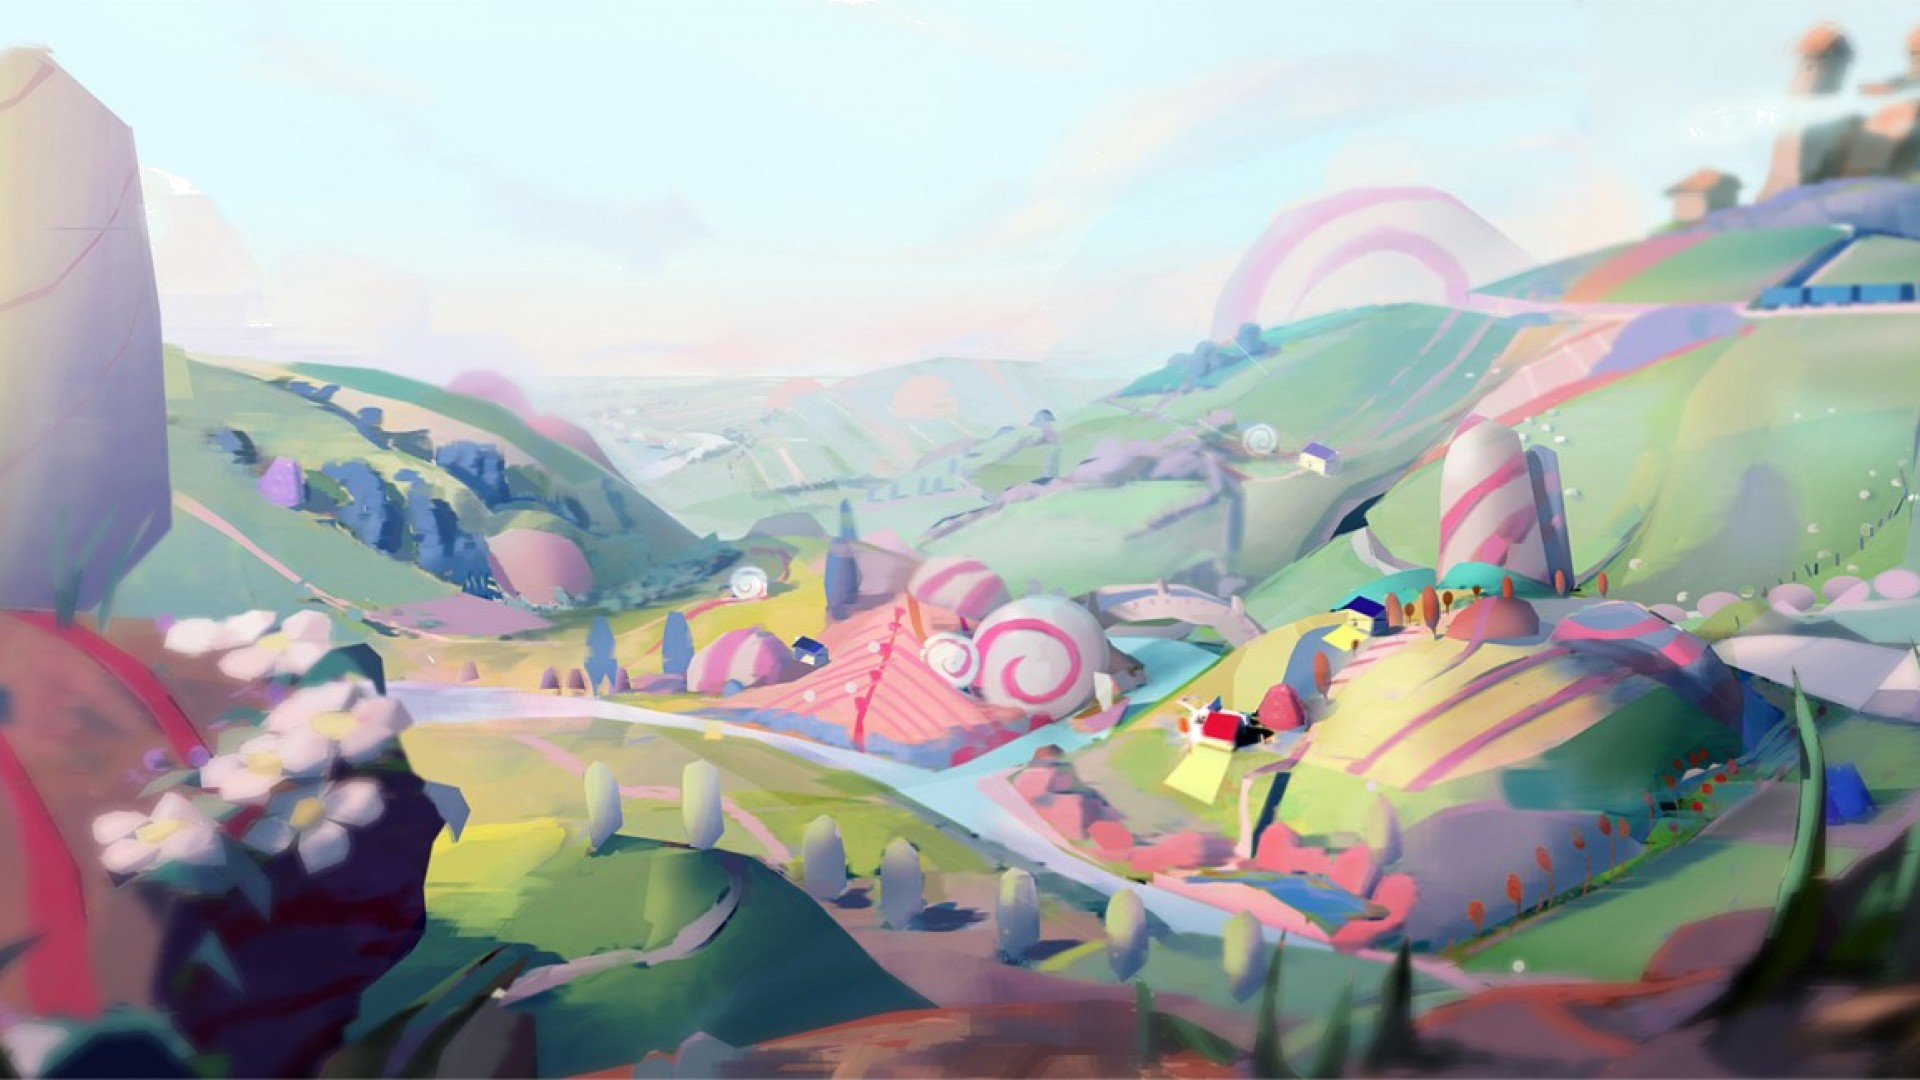
\includegraphics[width=\paperwidth,height=\paperheight]{demoland.png}}%
	\begin{frame}
	\frametitle{Address Resolution}

	% Explain to them that with so many addresses, we need ways to resolve addresses

	% URL to IP nslookup

	% IP to MAC arp
	\end{frame}
}

\note{
	Explain to them that with so many addresses, we need ways to resolve addresses

	URL to IP nslookup

	IP to MAC arp

	You may need to run nmap on local network to buff up arp table. I recommend doing it in this order

	arp Show that there are just a few entries

	nmap 192.168.1.1/24 

	replace IP address with current IP
	
		arp

	Show that there are many more entries 
}

\begin{frame}
	\frametitle{Why envelopes within envelopes...}

	\centering
    
  	\includegraphics<1>[width = \textwidth, height = .85\textheight, keepaspectratio]{figures/f1-4.png}

\end{frame}


\begin{colorframe}[black]

	\centering
	\Large
	Why bother with layers? What is the advantage?

\end{colorframe}

\note{	
	It allows abstracting away complexities of the communication
	From a programmers perspective, all he needs to do is deal with TCP/IP protocol
	and he can forget about the intricacies of how the signals are encoded and such

	Each layer can house multiple protocols. These protocols handle mundane details
	Since each interface is standard, we don't need to know the details. 
	But we can still chain different technologies together to get data to where it needs to be.

	It allows you to change protocols in each layer without disrupting the whole.
	This is the reason why a 40 year old idea can keep up with latest advances.

	Perhaps talk a bit about how IPv4 is being replaced under our noses.}





\end{document}
